\documentclass[aspectratio=169]{beamer}

\usepackage[utf8]{inputenc}
\usepackage{booktabs,geometry,microtype,xcolor,listings,graphicx}

\lstset{basicstyle=\footnotesize}

\title{SQL 101}
\author{Ethan Kent}
\institute{Spoonflower}
\date{\today}



\begin{document}

\frame{\titlepage}

\begin{frame}
  \frametitle{What is SQL?}
  \begin{itemize}
    \item SQL is a programming language for interacting with relational databases.
    \item It stands for \emph{S}tructured \emph{Q}uery
          \emph{L}anguage.\footnote{Or maybe it doesn't: ``It's a common
            misconception that \textit{SQL} stands for \textit{structured query
              language}; it stands for S-Q-L and nothing else. Why? Because ISO
            says so.'' Chris Fehily, \textit{SQL Database Programming} at loc'n
            222 (2015 Kindle ed.)}
    \item It was invented in 1974, and became a standard of ANSI and ISO in
          the late-1980s.
    \item Standards for SQL are now defined by ISO/IEC, though it appears that
          no actual SQL versions are compliant with all and only the ISO/IEC
          standards.
  \end{itemize}
\end{frame}

\begin{frame}
  \frametitle{What is a Relational Database?}
  \begin{itemize}
    \item A database (imperfectly) implements a \textit{relational model} of
          data, which is a mathematical model describing certain data
          structures and relationships.
    \item From an practical engineering perspective, a relational database
          has rows and columns, where each row is an entry in the database; and
          each column is a bit of data about that entry that matches the type
          required for that column.
    \item A relational database contrasts with NoSQL databases like MongoDB,
          in which users can insert free-form data that does not comprise
          rows of data in typed columns.
  \end{itemize}
\end{frame}

\begin{frame}
  \frametitle{What's up with MySQL, PostgreSQL, Microsoft SQL Server, Oracle, IBM DB2,~\ldots}
  \begin{itemize}
    \item The situation is similar to the existence of many programming
          languages aimed at the same problem domains.
    \item Some are open-source, some aren't.
    \item Some are more compliant with ISO/IEC standards (e.g. PostgreSQL);
          some are less so (e.g. SQLite).
    \item Some are part of ecosystems, are cloud-based/SaaS, etc. (e.g. Microsoft SQL
          Server, Amazon RDS, Google Cloud SQL).
  \end{itemize}
\end{frame}

\begin{frame}
  \frametitle{What does ``relational'' mean?}
  \framesubtitle{Spreadsheet analogy}

  You've probably encountered this problem if you've used a spreadsheet to
  keep track of things. It starts out simple:

  \begin{table}[]
    \begin{tabular}{@{}ll@{}}
      \toprule
      Person  & Age \\ \midrule
      Ethan   & 39  \\
      Madigan & 39  \\
      Belle   & 9   \\
      Milo    & 7   \\
      Clara   & 3   \\ \bottomrule
    \end{tabular}
  \end{table}
\end{frame}

\begin{frame}
  \frametitle{What does ``relational'' mean?}
  \framesubtitle{Spreadsheet analogy (cont'd)}

  Now we add a bit:

  \begin{table}[]
    \begin{tabular}{@{}lll@{}}
      \toprule
      Person  & Age & Favorite Dessert       \\ \midrule
      Ethan   & 39  & Oreo Cookies           \\
      Madigan & 39  & Klondike Bar           \\
      Belle   & 9   & Mint Chip Ice Cream    \\
      Milo    & 7   & Cookie Dough Ice Cream \\
      Clara   & 3   & Chocolate Ice Cream    \\ \bottomrule
    \end{tabular}
  \end{table}
\end{frame}

\begin{frame}
  \frametitle{What does ``relational'' mean?}
  \framesubtitle{Spreadsheet analogy (cont'd)}

  And now it turns out one person can't decide and has \emph{two} favorites.
  We could do this:

  \begin{table}[]
    \small
    \begin{tabular}{@{}lll@{}}
      \toprule
      Person  & Age & Favorite Dessert                  \\ \midrule
      Ethan   & 39  & Oreo Cookies, Mint Chip Ice Cream \\
      Madigan & 39  & Klondike Bar                      \\
      Belle   & 9   & Mint Chip Ice Cream               \\
      Milo    & 7   & Cookie Dough Ice Cream            \\
      Clara   & 3   & Chocolate Ice Cream               \\ \bottomrule
    \end{tabular}
  \end{table}

  Or maybe we try this:

  \begin{table}[]
    \small
    \begin{tabular}{@{}llll@{}}
      \toprule
      Person  & Age & Favorite Dessert \#1   & Favorite Dessert \# 2 \\ \midrule
      Ethan   & 39  & Oreo Cookies           & Mint Chip Ice Cream   \\
      Madigan & 39  & Klondike Bar           &                       \\
      Belle   & 9   & Mint Chip Ice Cream    &                       \\
      Milo    & 7   & Cookie Dough Ice Cream &                       \\
      Clara   & 3   & Chocolate Ice Cream    &                       \\ \bottomrule
    \end{tabular}
  \end{table}
\end{frame}

\begin{frame}
  \frametitle{What does ``relational'' mean?}
  \framesubtitle{Spreadsheet analogy (cont'd)}

  What's wrong with this?
  \begin{itemize}
    \item The comma-separated list is bad because---
          \begin{itemize}
            \item We can't sort or group things together, and
            \item The value has to be manipulated to be used.
          \end{itemize}
    \item The use of additional columns is bad because---
          \begin{itemize}
            \item We have to keep adding columns based on the data, so we're
                  never sure we're done with the structure of the database; and
            \item We are treating like things differently: columns mean the same
                  thing, but are distinct.
          \end{itemize}
  \end{itemize}
\end{frame}

\begin{frame}
  \frametitle{What does ``relational'' mean?}
  \framesubtitle{Spreadsheet analogy (cont'd)}

  So we do this:

  \begin{table}[]
    \small
    \begin{tabular}{@{}lll@{}}
      \toprule
      Person  & Age & Favorite Dessert       \\ \midrule
      Ethan   & 39  & Oreo Cookies           \\
      Ethan   & 39  & Mint Chip Ice Cream    \\
      Madigan & 39  & Klondike Bar           \\
      Belle   & 9   & Mint Chip Ice Cream    \\
      Milo    & 7   & Cookie Dough Ice Cream \\
      Clara   & 3   & Chocolate Ice Cream    \\ \bottomrule
    \end{tabular}
  \end{table}
\end{frame}

\begin{frame}
  \frametitle{What does ``relational'' mean?}
  \framesubtitle{Spreadsheet analogy (cont'd)}

  And now we want to have more detail about the desserts:

  \begin{table}[]
    \small
    \begin{tabular}{@{}llll@{}}
      \toprule
      Person  & Age & Favorite Dessert & Dessert Type      \\ \midrule
      Ethan   & 39  & Oreos            & Cookie            \\
      Ethan   & 39  & Mint Chip        & Ice Cream         \\
      Madigan & 39  & Klondike Bar     & Ice Cream Novelty \\
      Belle   & 9   & Mint Chip        & Ice Cream         \\
      Milo    & 7   & Cookie Dough     & Ice Cream         \\
      Clara   & 3   & Chocolate        & Ice Cream         \\ \bottomrule
    \end{tabular}
  \end{table}
\end{frame}

\begin{frame}
  \frametitle{What does ``relational'' mean?}
  \framesubtitle{Spreadsheet analogy (cont'd)}

  At this point we might feel queasy:
  \begin{itemize}
    \item We're repeating ourselves---
          \begin{itemize}
            \item Once we know the person is \textit{Ethan}, we know we have
                  a 39-year-old person.
            \item Once we know the dessert is \textit{Mint Chip}, we know we
                  have an \textit{Ice Cream}.
          \end{itemize}
    \item We have have data about different stuff in the same place.
  \end{itemize}
\end{frame}

\begin{frame}
  \frametitle{What does ``relational'' mean?}
  \framesubtitle{Spreadsheet analogy (cont'd)}

  Repeating ourselves is more than an inconvenience. Consider this:

  \begin{table}[]
    \small
    \begin{tabular}{@{}llll@{}}
      \toprule
      Person  & Age & Favorite Dessert & Dessert Type      \\ \midrule
      Ethan   & 39  & Oreos            & Cookie            \\
      Ethan   & 38  & Mint Chip        & Ice Cream         \\
      Madigan & 39  & Klondike Bar     & Ice Cream Novelty \\
      Belle   & 9   & Mint Chip        & Candy Bar         \\
      Milo    & 7   & Cookie Dough     & Ice Cream         \\
      Clara   & 3   & Chocolate        & Ice Cream         \\ \bottomrule
    \end{tabular}
  \end{table}


  \begin{itemize}
    \item Are these two desserts with the same name (``Mint Chip'')?
    \item Are there two \textit{Ethan}s?
    \item Are there mistakes?
    \item If there are mistakes, is Ethan 38 or 39? Is Mint Chip an Ice Cream
          or a Candy Bar?
  \end{itemize}
\end{frame}


\begin{frame}
  \frametitle{What does ``relational'' mean?}
  \framesubtitle{Spreadsheet analogy (cont'd)}

  So let's split things into different tables. And let's use some arbitrary,
  unique ``ID''s, so we can talk about a particular row without having to use
  some of the data (that could change):

  \begin{columns}[T]
    \begin{column}{0.3\textwidth}
      \noindent
      \begin{table}[]
        \footnotesize
        \begin{tabular}{@{}lll@{}}
          \toprule
          ID & Person  & Age \\ \midrule
          1  & Ethan   & 39  \\
          2  & Madigan & 39  \\
          3  & Belle   & 9   \\
          4  & Milo    & 7   \\
          5  & Clara   & 3   \\ \bottomrule
        \end{tabular}
      \end{table}
    \end{column}
    \begin{column}{0.5\textwidth}
      \begin{table}[]
        \footnotesize
        \begin{tabular}{@{}lll@{}}
          \toprule
          ID & Dessert      & Dessert Type      \\ \midrule
          1  & Oreos        & Cookies           \\
          2  & Mint Chip    & Ice Cream         \\
          3  & Klondike Bar & Ice Cream Novelty \\
          4  & Cookie Dough & Ice cream         \\
          5  & Chocolate    & Ice Cream         \\ \bottomrule
        \end{tabular}
      \end{table}
    \end{column}
  \end{columns}

  \vspace{1em}

  But now how can we show the relationship between these? Wait, did I just
  say \emph{relationship}? As in \emph{relational database}? Holy cow.
\end{frame}

\begin{frame}
  \frametitle{What does ``relational'' mean?}
  \framesubtitle{Spreadsheet analogy (cont'd)}
  \begin{columns}[T]
    \begin{column}{0.3\textwidth}
      \noindent
      \begin{table}[]
        \footnotesize
        \begin{tabular}{@{}lll@{}}
          \toprule
          ID & Person  & Age \\ \midrule
          1  & Ethan   & 39  \\
          2  & Madigan & 39  \\
          3  & Belle   & 9   \\
          4  & Milo    & 7   \\
          5  & Clara   & 3   \\ \bottomrule
        \end{tabular}
      \end{table}
    \end{column}
    \begin{column}{0.5\textwidth}
      \begin{table}[]
        \footnotesize
        \begin{tabular}{@{}lll@{}}
          \toprule
          ID & Dessert      & Dessert Type      \\ \midrule
          1  & Oreos        & Cookies           \\
          2  & Mint Chip    & Ice Cream         \\
          3  & Klondike Bar & Ice Cream Novelty \\
          4  & Cookie Dough & Ice cream         \\
          5  & Chocolate    & Ice Cream         \\ \bottomrule
        \end{tabular}
      \end{table}
    \end{column}
  \end{columns}

  \begin{table}[]
    \footnotesize
    \begin{tabular}{@{}ll@{}}
      \toprule
      Person ID & Dessert ID \\ \midrule
      1         & 1          \\
      1         & 2          \\
      2         & 3          \\
      3         & 2          \\
      4         & 4          \\
      5         & 5          \\ \bottomrule
    \end{tabular}
  \end{table}
\end{frame}

\begin{frame}
  \frametitle{What does ``relational'' mean?}
  \framesubtitle{Spreadsheet analogy (cont'd)}

  Did you notice the error that will bite us later? Cookie Dough is an ``Ice cream,'' not an ``Ice
  Cream.'' Let's fix that:

  \begin{columns}[T]
    \begin{column}{0.3\textwidth}
      \begin{table}[]
        \footnotesize
        \begin{tabular}{@{}lll@{}}
          \toprule
          ID & Person  & Age \\ \midrule
          1  & Ethan   & 39  \\
          2  & Madigan & 39  \\
          3  & Belle   & 9   \\
          4  & Milo    & 7   \\
          5  & Clara   & 3   \\ \bottomrule
        \end{tabular}
      \end{table}
    \end{column}
    \begin{column}{0.5\textwidth}
      \begin{table}[]
        \footnotesize
        \begin{tabular}{@{}ll@{}}
          \toprule
          ID & Desert Type       \\ \midrule
          1  & Cookie            \\
          2  & Ice Cream         \\
          3  & Ice Cream Novelty \\ \bottomrule
        \end{tabular}
      \end{table}
    \end{column}
  \end{columns}

  \begin{columns}[T]
    \begin{column}{0.3\textwidth}
      \begin{table}[]
        \footnotesize
        \begin{tabular}{@{}llp{5em}@{}}
          \toprule
          ID & Dessert      & Dessert Type ID \\ \midrule
          1  & Oreos        & 1               \\
          2  & Mint Chip    & 2               \\
          3  & Klondike Bar & 3               \\
          4  & Cookie Dough & 2               \\
          5  & Chocolate    & 2               \\ \bottomrule
        \end{tabular}
      \end{table}
    \end{column}
    \begin{column}{0.5\textwidth}
      \begin{table}[]
        \footnotesize
        \begin{tabular}{@{}ll@{}}
          \toprule
          Person ID & Dessert ID \\ \midrule
          1         & 1          \\
          1         & 2          \\
          2         & 3          \\
          3         & 2          \\
          4         & 4          \\
          5         & 5          \\ \bottomrule
        \end{tabular}
      \end{table}
    \end{column}
  \end{columns}
\end{frame}

\begin{frame}
  \frametitle{What does ``relational'' mean?}
  \framesubtitle{Spreadsheet analogy (cont'd)}

  What does any of this have to do with anything? Well, you've just seen
  examples of:

  \begin{itemize}
    \item Relational database design
    \item Foreign keys
    \item Primary keys
    \item Composite primary keys
    \item Join tables
    \item First and Third Normal Form
  \end{itemize}
\end{frame}

\begin{frame}
  \frametitle{Primary keys}

  \begin{columns}[T]
    \begin{column}{0.3\textwidth}
      \begin{table}[]
        \footnotesize
        \begin{tabular}{@{}lll@{}}
          \toprule
          ID                  & Person  & Age \\ \midrule
          \textcolor{blue}{1} & Ethan   & 39  \\
          \textcolor{blue}{2} & Madigan & 39  \\
          \textcolor{blue}{3} & Belle   & 9   \\
          \textcolor{blue}{4} & Milo    & 7   \\
          \textcolor{blue}{5} & Clara   & 3   \\ \bottomrule
        \end{tabular}
      \end{table}
    \end{column}
    \begin{column}{0.5\textwidth}
      \begin{table}[]
        \footnotesize
        \begin{tabular}{@{}ll@{}}
          \toprule
          ID              & Desert Type       \\ \midrule
          \color{blue}{1} & Cookie            \\
          \color{blue}{2} & Ice Cream         \\
          \color{blue}{3} & Ice Cream Novelty \\ \bottomrule
        \end{tabular}
      \end{table}
    \end{column}
  \end{columns}

  \begin{columns}[T]
    \begin{column}{0.3\textwidth}
      \begin{table}[]
        \footnotesize
        \begin{tabular}{@{}llp{5em}@{}}
          \toprule
          ID              & Dessert      & Dessert Type ID \\ \midrule
          \color{blue}{1} & Oreos        & 1               \\
          \color{blue}{2} & Mint Chip    & 2               \\
          \color{blue}{3} & Klondike Bar & 3               \\
          \color{blue}{4} & Cookie Dough & 2               \\
          \color{blue}{5} & Chocolate    & 2               \\ \bottomrule
        \end{tabular}
      \end{table}
    \end{column}
    \begin{column}{0.5\textwidth}
      \begin{table}[]
        \footnotesize
        \begin{tabular}{@{}ll@{}}
          \toprule
          Person ID         & Dessert ID        \\ \midrule
          \color{purple}{1} & \color{purple}{1} \\
          \color{purple}{1} & \color{purple}{2} \\
          \color{purple}{2} & \color{purple}{3} \\
          \color{purple}{3} & \color{purple}{2} \\
          \color{purple}{4} & \color{purple}{4} \\
          \color{purple}{5} & \color{purple}{5} \\ \bottomrule
        \end{tabular}
      \end{table}
    \end{column}
  \end{columns}
\end{frame}

\begin{frame}
  \frametitle{Foreign keys}

  \begin{table}
    \footnotesize
    \begin{tabular}[T]{@{}lll@{}}
      \toprule
      ID & Dessert      & Dessert Type ID \\ \midrule
      1  & Oreos        & \color{red}{1}  \\
      2  & Mint Chip    & \color{red}{2}  \\
      3  & Klondike Bar & \color{red}{3}  \\
      4  & Cookie Dough & \color{red}{2}  \\
      5  & Chocolate    & \color{red}{2}  \\ \bottomrule
    \end{tabular}
  \end{table}
  \begin{table}[]
    \footnotesize
    \begin{tabular}{@{}ll@{}}
      \toprule
      Person ID         & Dessert ID        \\ \midrule
      \color{purple}{1} & \color{purple}{1} \\
      \color{purple}{1} & \color{purple}{2} \\
      \color{purple}{2} & \color{purple}{3} \\
      \color{purple}{3} & \color{purple}{2} \\
      \color{purple}{4} & \color{purple}{4} \\
      \color{purple}{5} & \color{purple}{5} \\ \bottomrule
    \end{tabular}
  \end{table}
\end{frame}

\begin{frame}
  \frametitle{Composite primary keys}
  \begin{table}[]
    \footnotesize
    \begin{tabular}{@{}ll@{}}
      \toprule
      Person ID         & Dessert ID        \\ \midrule
      \color{purple}{1} & \color{purple}{1} \\
      \color{purple}{1} & \color{purple}{2} \\
      \color{purple}{2} & \color{purple}{3} \\
      \color{purple}{3} & \color{purple}{2} \\
      \color{purple}{4} & \color{purple}{4} \\
      \color{purple}{5} & \color{purple}{5} \\ \bottomrule
    \end{tabular}
  \end{table}
\end{frame}

\begin{frame}
  \frametitle{Join tables}
  \begin{table}[]
    \footnotesize
    \begin{tabular}{@{}ll@{}}
      \toprule
      Person ID & Dessert ID \\ \midrule
      1         & 1          \\
      1         & 2          \\
      2         & 3          \\
      3         & 2          \\
      4         & 4          \\
      5         & 5          \\ \bottomrule
    \end{tabular}
  \end{table}
\end{frame}

\begin{frame}
  \frametitle{First Normal Form}

  Don't do either of these things (columns must be ``atomic'' and there
  mustn't be ``repeating groups''):

  \begin{table}[]
    \footnotesize
    \begin{tabular}{@{}lll@{}}
      \toprule
      Person  & Favorite Dessert \\ \midrule
      Ethan   & Oreos, Mint Chip \\
      Madigan & Klondike Bar     \\
      Belle   & Mint Chip        \\
      Milo    & Cookie Dough     \\ \bottomrule
    \end{tabular}
  \end{table}

  \begin{table}[]
    \footnotesize
    \begin{tabular}{@{}llll@{}}
      \toprule
      Person  & Favorite Dessert \#1 & Favorite Dessert \# 2 \\ \midrule
      Ethan   & Oreos                & Mint Chip             \\
      Madigan & Klondike Bar         &                       \\
      Belle   & Mint Chip            &                       \\
      Milo    & Cookie Dough         &                       \\ \bottomrule
    \end{tabular}
  \end{table}
\end{frame}



\begin{frame}
  \frametitle{Third Normal Form}
  Don't do this:

  \begin{itemize}
    \item If we know \textit{Ethan}, then we automatically know
          \textit{39}; and
    \item If we know \textit{Mint Chip}, then we automatically
          know \textit{Ice Cream}:\footnote{In First and Second Normal Forms
            and no ``transitive dependencies.'' Second Normal Form has to do
            with composite primary keys, but it's impossible with the tables
            we've looked at so far.}
  \end{itemize}

  \begin{table}[]
    \footnotesize
    \begin{tabular}{@{}llll@{}}
      \toprule
      Person  & Age & Favorite Dessert & Dessert Type      \\ \midrule
      Ethan   & 39  & Oreos            & Cookie            \\
      Ethan   & 39  & Mint Chip        & Ice Cream         \\
      Madigan & 39  & Klondike Bar     & Ice Cream Novelty \\
      Belle   & 9   & Mint Chip        & Ice Cream         \\
      Milo    & 7   & Cookie Dough     & Ice Cream         \\
      Clara   & 3   & Chocolate        & Ice Cream         \\ \bottomrule
    \end{tabular}
  \end{table}

\end{frame}

\begin{frame}[fragile]
  \frametitle{Create some tables}

  \begin{lstlisting}
CREATE TABLE people (
  id SERIAL NOT NULL,
  name TEXT NOT NULL UNIQUE,
  age INTEGER NOT NULL,
  PRIMARY KEY (id)
);

CREATE TABLE dessert_types (
  id SERIAL NOT NULL,
  name TEXT NOT NULL UNIQUE,
  PRIMARY KEY (id)
);
  \end{lstlisting}
\end{frame}

\begin{frame}[fragile]
  \frametitle{Create some more tables}

  \begin{lstlisting}
CREATE TABLE desserts (
  id SERIAL NOT NULL,
  name TEXT NOT NULL UNIQUE,
  dessert_type_id INTEGER NOT NULL,
  PRIMARY KEY (id),
  FOREIGN KEY (dessert_type_id)
    REFERENCES dessert_types(id)
);

CREATE TABLE people_desserts (
  person_id INTEGER NOT NULL,
  dessert_id INTEGER NOT NULL,
  PRIMARY KEY (person_id, dessert_id),
  FOREIGN KEY (person_id) REFERENCES people(id),
  FOREIGN KEY (dessert_id) REFERENCES desserts(id)
);

  \end{lstlisting}

\end{frame}


\begin{frame}[fragile]
  \frametitle{Insert some data}
  \begin{lstlisting}
INSERT INTO people (name, age) VALUES
  ('Ethan', 39),
  ('Madigan', 39),
  ('Belle', 9),
  ('Milo', 7),
  ('Clara', 3);

INSERT INTO dessert_types (name) VALUES
  ('Cookie'),
  ('Ice Cream'),
  ('Ice Cream Novelty');
  \end{lstlisting}
\end{frame}

\begin{frame}[fragile]
  \frametitle{Now what?}
  \begin{lstlisting}
INSERT INTO desserts (dessert_name, dessert_type_id) VALUES
  -- ('Oreos', ???),
  \end{lstlisting}
\end{frame}

\begin{frame}[fragile]
  \frametitle{Queries!}
  \begin{lstlisting}
INSERT INTO desserts (name, dessert_type_id) VALUES
  ('Oreos',
    (SELECT id FROM dessert_types
     WHERE name = 'Cookie')),

  ('Mint Chip',
    (SELECT id FROM dessert_types
     WHERE name = 'Ice Cream')),

  ('Klondike Bar',
    (SELECT id FROM dessert_types
     WHERE name = 'Ice Cream Novelty')),

  ('Cookie Dough',
    (SELECT id FROM dessert_types
     WHERE name = 'Ice Cream')),

  ('Chocolate',
    (SELECT id FROM dessert_types
     WHERE name = 'Ice Cream'));
  \end{lstlisting}
\end{frame}

\begin{frame}[fragile]
  \frametitle{Not very DRY. How about a CTE?}
  \begin{lstlisting}
WITH
  cookie_id AS
    (SELECT id FROM dessert_types
     WHERE dessert_type = 'Cookie'),
  ice_cream_id AS
    (SELECT id FROM dessert_types
     WHERE dessert_type = 'Ice Cream'),
  ice_cream_novelty_id AS
    (SELECT id FROM dessert_types
     WHERE dessert_type = 'Ice Cream Novelty')
INSERT INTO desserts (dessert_name, dessert_type_id) VALUES
  ('Oreos', (SELECT id FROM cookie_id)),
  ('Mint Chip', (SELECT id FROM ice_cream_id)),
  ('Klondike Bar', (SELECT id FROM ice_cream_novelty_id)),
  ('Cookie Dough', (SELECT id FROM ice_cream_id)),
  ('Chocolate', (SELECT id FROM ice_cream_id));

  \end{lstlisting}
\end{frame}

\begin{frame}[fragile]
  \frametitle{Not very DRY. How about a CTE?}
  Not with MySQL though.
\end{frame}

\begin{frame}[fragile]
  \frametitle{Okay but we're getting ahead of ourselves!}

  We're doing CTEs and we haven't even done queries. What is wrong with you?
\end{frame}

\begin{frame}[fragile]
  \frametitle{Okay but we're getting ahead of ourselves!}

  There's a bootstrapping issue: we need a database to do some database
  stuff. It's like languages where doing ``Hello world'' is
  hard.\footnote{I'm looking at you Haskell.}
\end{frame}

\begin{frame}[fragile]
  \frametitle{Baseball example}

  For our German friends, baseball is an American sport that's a bit like
  cricket, though actually comprehensible. There are 30 teams divided into
  two leagues,\footnote{Technically, only one of the leagues plays baseball;
    the other plays a game that appears on the surface like baseball but that
    is not actually baseball, as it involves the Designated Hitter rule.} and
  each team plays 162 games per year. Because of the number of games and
  long history, baseball is big among statisticians.
  \begin{center}
    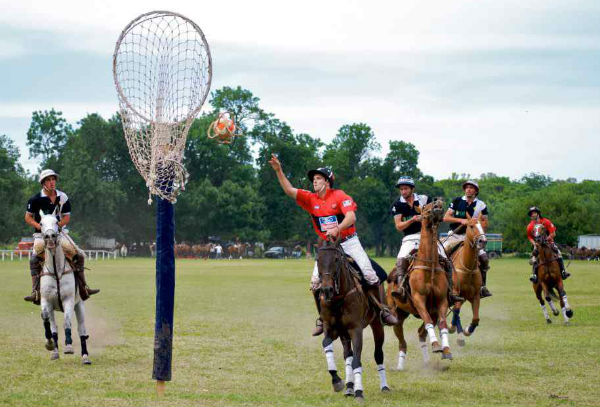
\includegraphics[width=0.5\textheight]{Pato.jpg}
  \end{center}
\end{frame}


\begin{frame}[fragile]
  \frametitle{Baseball example}

  I have a rudimentary database of 2016 MLB info: just games, teams, and
  players. Let's figure out the following:

  \begin{enumerate}
    \item What player has the id 'dillp101'?\label{pickles}
    \item How many teams were there in 2016?\label{num_teams}
    \item How many players played in 2016?\label{num_players}
    \item How many games did Anthony Rizzo play in 2016?\label{rizzo}
    \item What is the commonest first name in MLB history?\label{common}
    \item What player played for the most teams (choose only one if it's a
          tie), and what teams were they?\label{most_teams}
    \item From those players who played at least 10 total games in 2016, what
          player played the highest percentage of night games?\label{night}
  \end{enumerate}
\end{frame}

\begin{frame}[fragile]
  \frametitle{Baseball example, answer \ref{pickles}}
  \begin{lstlisting}
SELECT * FROM players WHERE id = 'dillp101';
  \end{lstlisting}
\end{frame}

\begin{frame}[fragile]
  \frametitle{Baseball example, answer \ref{num_teams}}
  \begin{lstlisting}
SELECT COUNT(*) FROM teams;
  \end{lstlisting}
\end{frame}

\begin{frame}[fragile]
  \frametitle{Baseball example, answer \ref{num_players}}
  \begin{lstlisting}
SELECT COUNT(DISTINCT player_id) FROM players_teams;
  \end{lstlisting}
\end{frame}

\begin{frame}[fragile]
  \frametitle{Baseball example, answer \ref{rizzo}}
  \begin{lstlisting}
SELECT COUNT(pg.game_id)
FROM players player
INNER JOIN players_games pg
        ON player.id = pg.player_id
WHERE first = 'Anthony'
  AND last = 'Rizzo';
  \end{lstlisting}
\end{frame}

\begin{frame}[fragile]
  \frametitle{Baseball example, answer \ref{common}}
  \begin{lstlisting}
SELECT COUNT(first), first
FROM players
GROUP BY first
ORDER BY 1 DESC
LIMIT 1;
  \end{lstlisting}
\end{frame}

\begin{frame}[fragile]
  \frametitle{Baseball example, answer \ref{most_teams}}
  \begin{lstlisting}
SELECT sub.first AS "First Name",
       sub.last AS "Last Name",
       team.name AS "Team Name"
FROM (
  SELECT player.id,
         player.first,
         player.last,
         COUNT(pt.team_id)
  FROM players player
  INNER JOIN players_teams pt
          ON pt.player_id = player.id
  GROUP BY player.id
  ORDER BY 4 DESC
  LIMIT 1
) sub
INNER JOIN players_teams pt
        ON pt.player_id = sub.id
INNER JOIN teams team
        ON team.id = pt.team_id;
  \end{lstlisting}
\end{frame}

\begin{frame}[fragile]
  \frametitle{Baseball example, answer \ref{night}}
  \begin{lstlisting}
SELECT player.first,
       player.last,
       CAST(night_games.tally AS FLOAT) / total_games.tally AS "Percent"
FROM ( SELECT pg.player_id, COUNT(pg.player_id) AS tally
       FROM players_games pg
       INNER JOIN games game ON game.id = pg.game_id
       WHERE game.day_night = 'N'
       GROUP BY pg.player_id
) as night_games INNER JOIN (
       SELECT pg.player_id, COUNT(pg.player_id) AS tally
       FROM players_games pg
       INNER JOIN games game ON game.id = pg.game_id
       GROUP BY pg.player_id
) AS total_games ON night_games.player_id = total_games.player_id
INNER JOIN players player ON player.id = total_games.player_id
WHERE total_games.tally >= 10
ORDER BY "Percent" DESC
LIMIT 1;
  \end{lstlisting}
\end{frame}
\end{document}
